\section{Dữ liệu 1: Mô hình hồi quy đa biến}

\subsection*{Giới thiệu bộ dữ liệu}
Bộ dữ liệu được tìm thấy trên trang Kaggle - một cộng đồng trực tuyến về khoa học dữ liệu và học máy. Đó là bộ dữ liệu \textbf{Chi phí Y tế Cá nhân} \footnote{\url{https://www.kaggle.com/mirichoi0218/insurance}} (\textit{Medical Cost Personal Datasets}). Đây là một bộ dữ liệu được lấy ra từ cuốn \textit{Machine Learning with R} của Brett Lantz, một cuốn sách giới thiệu về học máy bằng R.

Bộ dữ liệu ghi lại các thông tin về thông tin của người đăng kí bảo hiểm và chi phí mà bảo hiểm y tế phải chi trả cho cá nhân đó. Bộ dữ liệu có 1338 quan trắc, gồm 7 biến sau:
\begin{enumerate}
	\item \texttt{age}: tuổi
	\item \texttt{sex}: giới tính
	\item \texttt{bmi}: chỉ số đo cân nặng, sử dụng tỷ lệ giữa cân nặng và chiều cao ($kg / m$), chỉ số BMI lý tưởng là từ 18.5 đến 24.9.
	\item \texttt{children}: số lượng trẻ em được bao gồm trong bảo hiểm y tế của người đăng kí.	
	\item \texttt{smoker}: 1 nếu người đó có hút thuốc, ngược lại là 0.
	\item \texttt{region}: vùng miền ở US, bao gồm Đông Bắc (\textit{northeast}), Đông Nam (\textit{southeast}), Tây Nam (\textit{southwest}), Tây Bắc (\textit{northwest}).
	\item \texttt{charges}: Chi phí y tế của cá nhân được chi trả bởi bảo hiểm y tế.
\end{enumerate}

Nhận thấy biến \texttt{region} có bốn giá trị, để thuận tiện cho việc hồi quy mô hình đa biến, chúng ta cần phải tách \texttt{region} thành ba biến giả lần lượt là \texttt{region\_ne} - vùng Đông Bắc, \texttt{region\_se} - vùng Đông Nam và \texttt{region\_sw} - vùng Tây Nam, nếu không nằm trong 3 vùng này thì nó là vùng Tây Bắc. Vậy bộ dữ liệu hiện tại có tất cả 9 biến.

Kiểm tra sự trùng lặp dữ liệu trong bộ dữ liệu, ta có kết quả từ phầm mềm R ở hình \ref{fig-a1:dataset-duplicated}, thấy rằng chỉ tồn tại một dữ liệu bị trùng, ta tiến hành loại bỏ dữ liệu này. Vậy bộ dữ liệu hiện tại có 1337 quan trắc.
\begin{figure}[H]
	\centering
	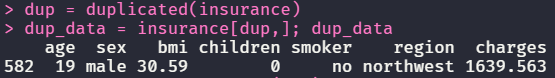
\includegraphics[width=0.7\linewidth]{images/A1/dataset-duplicated}
	\caption{Dữ liệu bị trùng lặp}
	\label{fig-a1:dataset-duplicated}
\end{figure}

Một vài quan trắc đầu tiên trong bộ dữ liệu được thể hiện trong hình \ref{fig-a1:head-dataset} và số chiều của nó: 1337 dòng (quan trắc) và 9 cột (biến).
\begin{figure}[H]
	\centering
	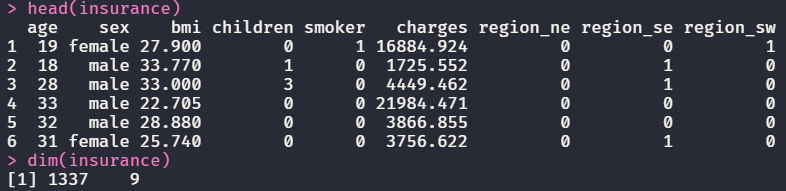
\includegraphics[width=0.8\linewidth]{images/A1/head-dataset}
	\caption{Một vài quan trắc đầu tiên và số chiều của bộ dữ liệu}
	\label{fig-a1:head-dataset}
\end{figure}

Phân bố của 7 biến ban đầu ở hình \ref{fig-a1:plot-vars} và trung bình tổng của từng biến theo biến phụ thuộc \texttt{charges} ở hình \ref{fig-a1:aggregate-vars}.
\begin{figure}[H]
	\centering
	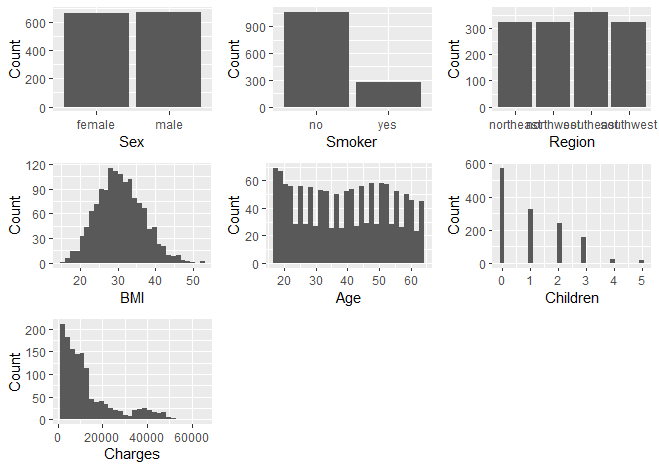
\includegraphics[width=0.8\linewidth]{images/A1/plot-vars}
	\caption{Phân bố của 7 biến ban đầu}
	\label{fig-a1:plot-vars}
\end{figure}

\begin{figure}[H]
	\centering
	\subfloat[\texttt{sex}]
	{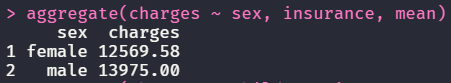
\includegraphics[width=0.6\linewidth]{images/A1/aggregate-sex}}\\
	\subfloat[\texttt{smoker}]
	{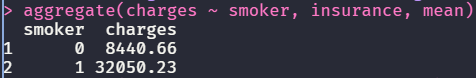
\includegraphics[width=0.65\linewidth]{images/A1/aggregate-smoker}}\\
	\subfloat[\texttt{region}]
	{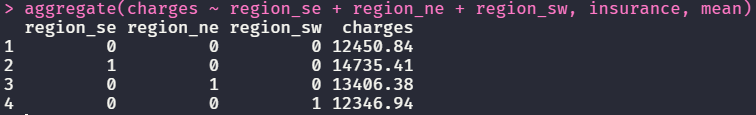
\includegraphics[width=0.9\linewidth]{images/A1/aggregate-region}}\\
	\subfloat[\texttt{bmi}]
	{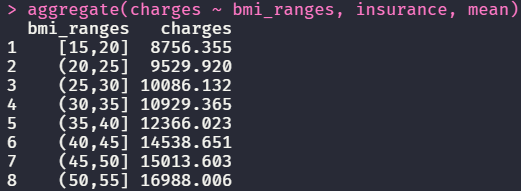
\includegraphics[width=0.7\linewidth]{images/A1/aggregate-bmi_ranges}}\\
	\subfloat[\texttt{age}]
	{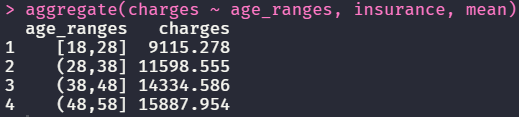
\includegraphics[width=0.65\linewidth]{images/A1/aggregate-age_ranges}}\\
	\subfloat[\texttt{children}]
	{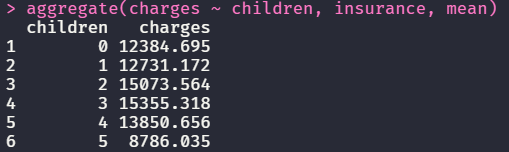
\includegraphics[width=0.65\linewidth]{images/A1/aggregate-children}}\\
	\caption{Trung bình tổng của từng biến theo biến phụ thuộc \texttt{charges}}
	\label{fig-a1:aggregate-vars}
\end{figure}

Một số điều thú vị thấy được ở hai hình \ref{fig-a1:plot-vars} và \ref{fig-a1:aggregate-vars}, ta xét lần lượt từng biến:
\begin{itemize}
	\item \texttt{sex}: dù là nam hay nữ thì phân bố giữa hai giới này đều xấp xỉ nhau, đồng thời chi phí trung bình mà bảo hiểm y tế chi trả cũng xấp xỉ nhau.
	\item \texttt{smoker}: số lượng người hút thuốc ít hơn số lượng người không hút thuốc có trong bộ dữ liệu, nhưng chi phí trung bình mà bảo hiểm y tế chi trả cho nhóm này thì hoàn toàn cao hơn rất nhiều, điều này khá hiển nhiên.
	\item \texttt{region}: phân bố của các vùng và chi phí trung bình mà bảo hiểm y tế chi trả ở từng vùng cũng đều xấp xỉ nhau. 
	\item \texttt{bmi}: chỉ số BMI có phân bố dạng chuẩn, và chi phí trung bình mà bảo hiểm y tế chi trả cũng tăng dần đều theo chỉ số này, điều này cũng hợp lý vì khi chỉ số BMI càng cao thì khả năng bị béo phì cũng tăng. 
	\item \texttt{age}: tuổi tác có phân bố ngẫu nhiên, và chi phí trung bình mà bảo hiểm y tế chi trả cũng tăng dần theo tuổi, điều này cũng khá hiển nhiên.
	\item \texttt{children}: phân bố của trẻ em được hưởng theo bảo hiểm bị lệch hẳn về bên trái, nên chi phí trung bình mà bảo hiểm y tế chi trả cho 4-5 trẻ em có thể bị sai lệch do mất cân bằng dữ liệu.
\end{itemize}

Nhận xét tổng quan, ta thấy rằng chi phí bảo hiểm y tế chi trả \texttt{charges} có khả năng phụ thuộc vào các đặc tính như người hút thuốc \texttt{smoker}, chỉ số \texttt{bmi}, tuổi tác \texttt{age} và số trẻ em phụ thuộc \texttt{children}. Các đặc tính còn lại như vùng miền \texttt{region} và giới tính \texttt{sex} có thể sẽ không ảnh hưởng nhiều đến \texttt{charges}.

\subsection*{Phân tích và chọn mô hình}

Xét mô hình đầy đủ sau:
\begin{equation}\label{a1-model-full}
	\begin{split}
		\texttt{charges} = \beta_0 + &\beta_1 \times \texttt{age} + \beta_2 \times \texttt{sex} + \beta_3 \times \texttt{bmi} + \beta_4 \times \texttt{children} + \beta_5 \times \texttt{smoker}\\ + &\beta_6 \times \texttt{region\_ne} + \beta_7 \times \texttt{region\_se} + \beta_8 \times \texttt{region\_sw} + \epsilon
	\end{split}
\end{equation}

Mô hình hồi quy đầy đủ có các thông số ở hình \ref{fig-a1:model-full}, đúng như dự đoán, biến vùng miền \texttt{region} và giới tính \texttt{sex} không có ý nghĩa thống kê, và các biến còn lại có ý nghĩa thống kê khá cao.
\begin{figure}[H]
	\centering
	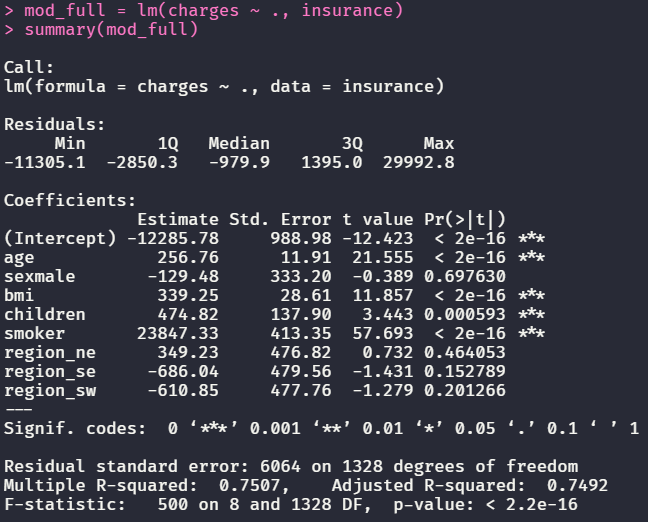
\includegraphics[width=0.7\linewidth]{images/A1/model-full}
	\caption{Mô hình đầy đủ}
	\label{fig-a1:model-full}
\end{figure}

Ta sử dụng phương pháp tính hệ số VIF để kiểm tra hiện tượng đa cộng tuyến có trong mô hình này, kết quả từ phần mềm R ở hình \ref{fig-a1:model-full-vif} cho thấy các chỉ số VIF đều dưới 5, chứng tỏ không tồn tại hiện tượng này trong mô hình.
\begin{figure}[H]
	\centering
	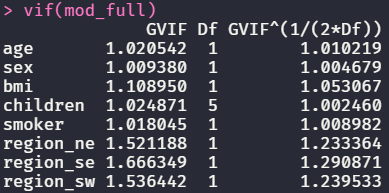
\includegraphics[width=0.6\linewidth]{images/A1/model-full-vif}
	\caption{Hiện tượng đa cộng tuyến có trong mô hình đầy đủ}
	\label{fig-a1:model-full-vif}
\end{figure}


\subsection*{Nhận xét và kết luận}